\SourceLeaf{326}%
% A544-P0326-D01
Inbegriff der Zahlen $f,f',f''$ etc. das System der Primitivreste von $m$. Ihre Anzahl ist immer $=aa+bb$.

% A544-P0326-D02
\Article{12}
Man kann das System der Primitivreste auf vielfache Art bilden; die einfachste ist, die Punkte innerhalb des Quadrats $0,m,(1+i)m,im$ zu wählen; dazu müssen aber noch hinzugefügt werden
\begin{enumerate}
\item[I.] der Punkt oder die Grösse $0$
\item[II.] alle Punkte auf zwei einander nicht gegenüberliegenden Grenzlinien.
\end{enumerate}
Anstatt auf einer der $4$ Grenzlinien alle Punkte zu nehmen, kann man sie auch auf mehren zugleich nehmen.

% A544-P0326-D03
Diese Auswahl dieser Punkte auf den Grenzlinien, falls welche darauf fallen, kann auf mehrfache Art geschehen, so dass obigen Bedingungen Genüge geschieht. Am einfachsten ist die folgende Manier.

% A544-P0326-D04
Man nehme auf der Grenzlinie $0,m$ alle Punkte zwischen $0$ und $\frac12m$ inclus. und auf der Grenzlinie $0,im$ alle Punkte von $\frac12im$ bis $im$ exclusive und auf ähnliche Art bei den beiden andern.

% A544-P0326-D05
Man kann diese beiden Manieren so sinnlich darstellen
\begin{center}\resizebox{.85\textwidth}{!}{\begin{tikzpicture}[x=1bp,y=-1bp,line cap=round,line join=round]
\path[use as bounding box] (0,0) rectangle (1230,440);
\begin{pgfinterruptboundingbox}
\draw[line width=2.2bp] (228,69) -- (72,214) -- (218,366) -- (373,219) -- (326,168);
\draw[line width=2.2bp] (322,163) -- (257,96);
\draw[line width=2.2bp] (250,90) -- (228,69);
\draw[line width=2bp] (148,136) circle[radius=5bp];
\draw[line width=2bp] (304,140) circle[radius=5bp];
\draw[line width=2bp] (297,284) circle[radius=5bp];
\draw[line width=2bp] (152,290) circle[radius=5bp];
\node[inner sep=0pt,outer sep=0pt,anchor=center] at (53,214) {\scalebox{3.5}{\ensuremath{m}}};
\node[inner sep=0pt,outer sep=0pt,anchor=center] at (228,48) {\scalebox{3.5}{\ensuremath{(1+i)m}}};
\node[inner sep=0pt,outer sep=0pt,anchor=center] at (399,220) {\scalebox{3.5}{\ensuremath{im}}};
\node[inner sep=0pt,outer sep=0pt,anchor=center] at (213,387) {\scalebox{3.5}{\ensuremath{0}}};
\draw[line width=2.2bp] (839,229) -- (993,77) -- (1143,234) -- (987,378) -- cycle;
\draw[line width=2bp] (878,197) circle[radius=5bp];
\draw[line width=2bp] (906,155) circle[radius=5bp];
\draw[line width=2bp] (951,112) circle[radius=5bp];
\draw[line width=2bp] (1023,116) circle[radius=5bp];
\draw[line width=2bp] (1069,151) circle[radius=5bp];
\draw[line width=2bp] (1112,193) circle[radius=5bp];
\draw[line width=2bp] (869,270) circle[radius=5bp];
\draw[line width=2bp] (915,303) circle[radius=5bp];
\draw[line width=2bp] (956,344) circle[radius=5bp];
\draw[line width=2bp] (984,373) circle[radius=5bp];
\draw[line width=2bp] (1024,352) circle[radius=5bp];
\draw[line width=2bp] (1055,309) circle[radius=5bp];
\draw[line width=2bp] (1098,269) circle[radius=5bp];
\node[inner sep=0pt,outer sep=0pt,anchor=center] at (819,229) {\scalebox{3.5}{\ensuremath{m}}};
\node[inner sep=0pt,outer sep=0pt,anchor=center] at (991,54) {\scalebox{3.5}{\ensuremath{(1+i)m}}};
\node[inner sep=0pt,outer sep=0pt,anchor=center] at (1166,236) {\scalebox{3.5}{\ensuremath{im}}};
\node[inner sep=0pt,outer sep=0pt,anchor=center] at (978,397) {\scalebox{3.5}{\ensuremath{0}}};
\end{pgfinterruptboundingbox}
\end{tikzpicture}
}\end{center}

% A544-P0326-D06
\Article{13}
Schliesst man von den Primitivpunkten aus
\begin{enumerate}
\item[I.] Bloss den Punkt $0$, wenn $a$ gerade und $b$ ungerade oder umgekehrt.
\item[II.] Die Punkte $0$ und $\frac12(1+i)m$, wenn $a$ und $b$ beide ungerade.
\item[III.] Die vier Punkte $0,\frac12m,\frac12(1+i)m,\frac12im$, wenn $a$ und $b$ beide gerade,
\end{enumerate}
so nennen wir die übrigbleibenden eigentliche Primitivpunkte, die ausgeschlossenen uneigentliche. Die Anzahl von jenen ist also
\[
\begin{array}{rrcl}
\text{in Fall}&\mathrm{I}&=&aa+bb-1\\
&\mathrm{II}&=&aa+bb-2\\
&\mathrm{III}&=&aa+bb-4
\end{array}
\]
also immer durch $4$ theilbar.

\SourceLeaf{327}%
% A544-P0327-D01
\Article{14}
Diese eigentlichen Primitivpunkte lassen sich in $4$ Classen $F,F',F'',F'''$ theilen, so dass
\[
\begin{array}{llll}
iF\equiv F'&iF'\equiv F''&iF''\equiv F'''&iF'''\equiv F\\
-F\equiv F''&-F'\equiv F'''&-F''\equiv F&-F'''\equiv F'\\
-iF\equiv F'''&-iF'\equiv F&-iF''\equiv F'&-iF'''\equiv F''
\end{array}
\]
Hiebei findet nun folgendes höchst wichtige Theorem statt.

% A544-P0327-D02
Es sei $M$ eine Zahl, welche mit $m$ keinen Factor gemein hat. Von den Zahlen $MF$ gehören in die Classe $F$ eine Anzahl von $n$
\[
\begin{array}{cc}F'&n'\\F''&n''\\F'''&n'''\end{array}
\]
und der kleinste Rest von $n'+2n''+3n''$ nach dem Modulus $4$ sei $=N$, also $N$ einer der $4$ Zahlen $0,1,2,3$ gleich: unter dieser Voraussetzung ist $N$ \emph{unabhängig} von der Art der Vertheilung der Primitivreste in Classen. Wir nennen ihn den Decident des biquadratischen Verhältnisses der Zahl $M$ zu $m$.

% A544-P0327-D03
\Article{15}
Die einfachste Art der Vertheilung ist allerdings folgende
\begin{center}\resizebox{.35\textwidth}{!}{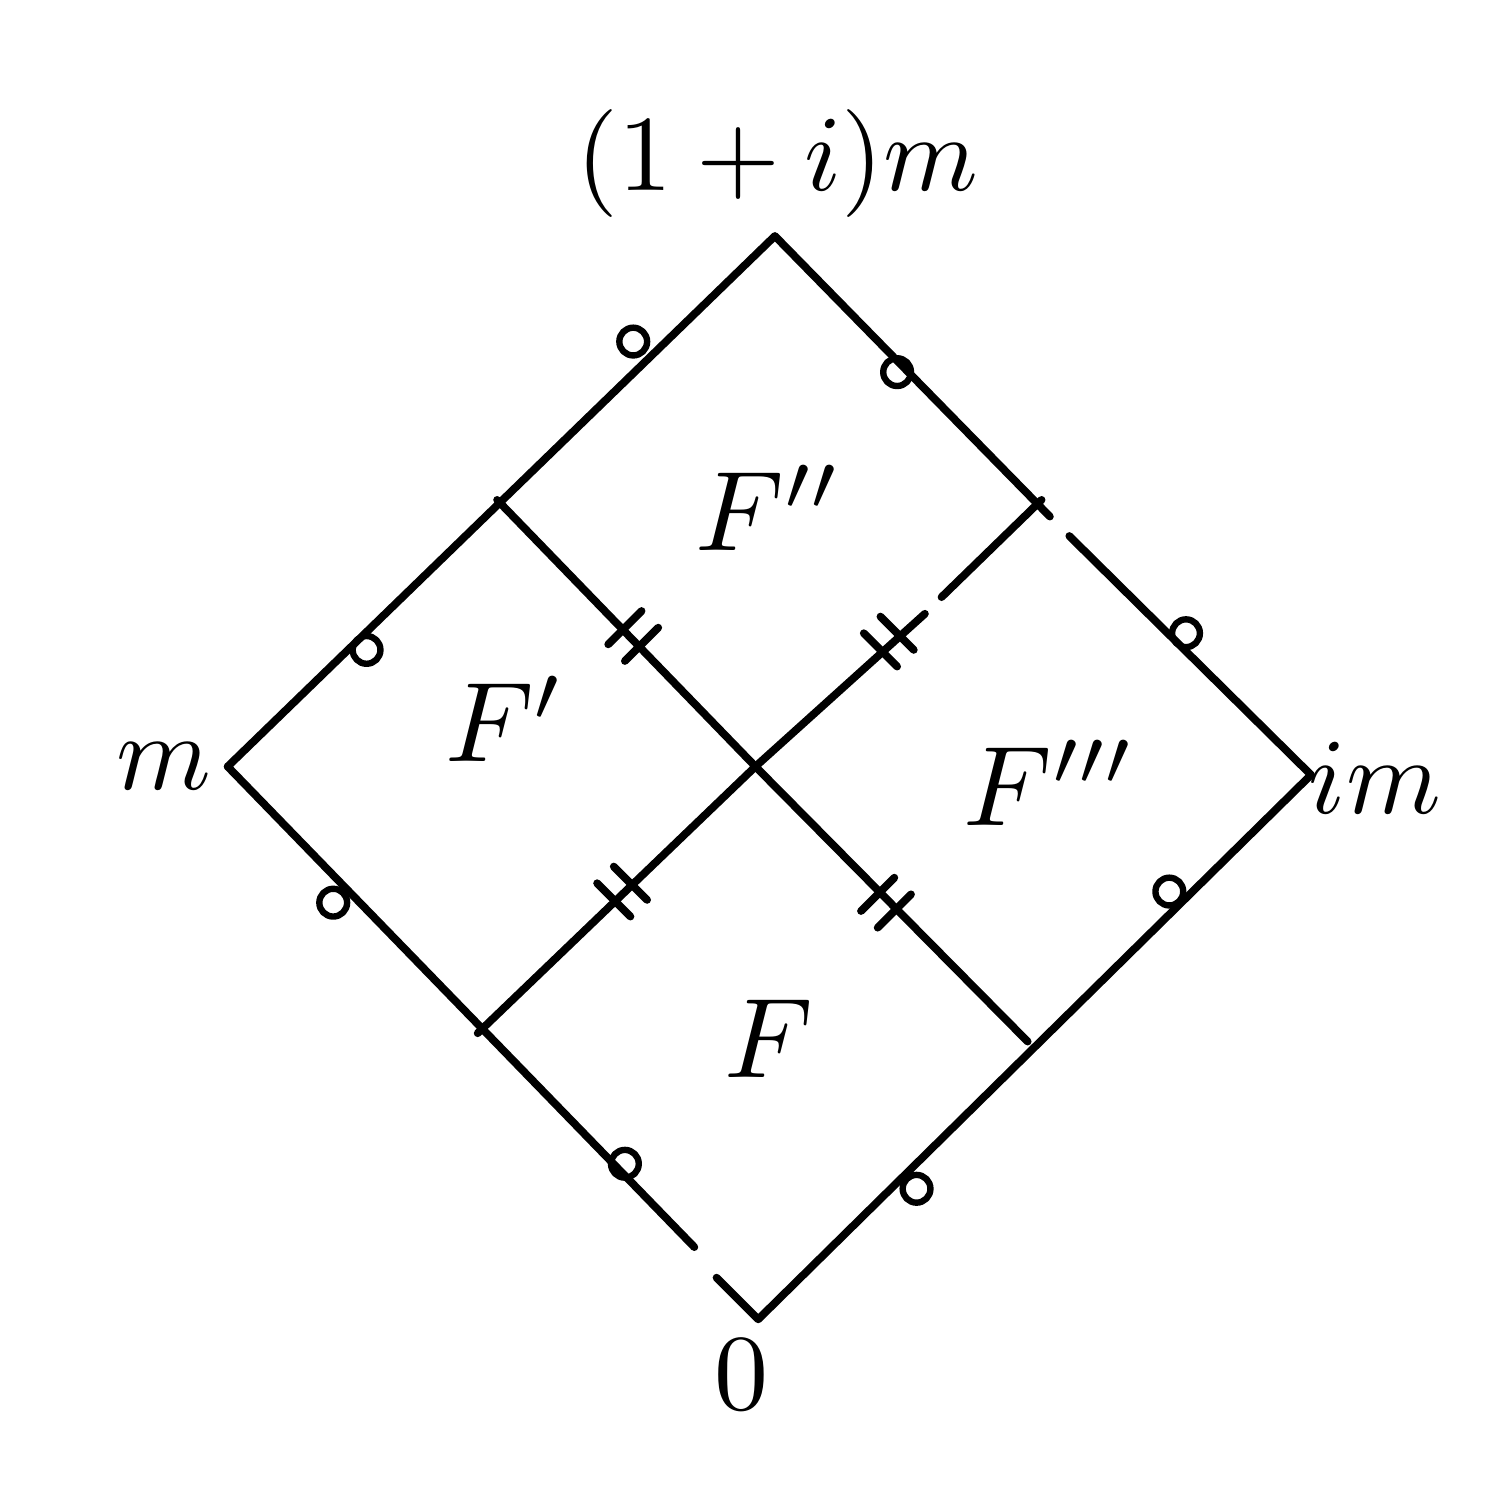
\begin{tikzpicture}[x=1bp,y=-1bp,line cap=round,line join=round]
\path[use as bounding box] (0,0) rectangle (520,520);
\begin{pgfinterruptboundingbox}
\draw[line width=2.8bp] (72,266) -- (269,75) -- (368,176);
\draw[line width=2.8bp] (375,183) -- (462,269) -- (263,465) -- (248,450);
\draw[line width=2.8bp] (240,439) -- (72,266);
\draw[line width=2.8bp] (169,170) -- (262,266) -- (360,365);
\draw[line width=2.8bp] (365,170) -- (329,205);
\draw[line width=2.8bp] (323,211) -- (262,266) -- (162,362);
\draw[line width=2.3bp] (218,113) circle[radius=5bp];
\draw[line width=2.3bp] (313,124) circle[radius=5bp];
\draw[line width=2.3bp] (122,224) circle[radius=5bp];
\draw[line width=2.3bp] (417,218) circle[radius=5bp];
\draw[line width=2.3bp] (110,315) circle[radius=5bp];
\draw[line width=2.3bp] (411,311) circle[radius=5bp];
\draw[line width=2.3bp] (215,409) circle[radius=5bp];
\draw[line width=2.3bp] (320,418) circle[radius=5bp];
\draw[line width=2.8bp] (209,222) -- (221,210);
\draw[line width=2.8bp] (215,228) -- (227,216);
\draw[line width=2.8bp] (301,218) -- (313,230);
\draw[line width=2.8bp] (307,212) -- (319,224);
\draw[line width=2.8bp] (205,308) -- (217,320);
\draw[line width=2.8bp] (211,302) -- (223,314);
\draw[line width=2.8bp] (300,318) -- (312,306);
\draw[line width=2.8bp] (306,324) -- (318,312);
\node[inner sep=0pt,outer sep=0pt,anchor=center] at (267,173) {\scalebox{4.1}{\ensuremath{F''}}};
\node[inner sep=0pt,outer sep=0pt,anchor=center] at (172,249) {\scalebox{4.1}{\ensuremath{F'}}};
\node[inner sep=0pt,outer sep=0pt,anchor=center] at (368,272) {\scalebox{4.1}{\ensuremath{F'''}}};
\node[inner sep=0pt,outer sep=0pt,anchor=center] at (267,364) {\scalebox{4.1}{\ensuremath{F}}};
\node[inner sep=0pt,outer sep=0pt,anchor=center] at (49,266) {\scalebox{3.9}{\ensuremath{m}}};
\node[inner sep=0pt,outer sep=0pt,anchor=center] at (270,49) {\scalebox{3.9}{\ensuremath{(1+i)m}}};
\node[inner sep=0pt,outer sep=0pt,anchor=center] at (485,270) {\scalebox{3.9}{\ensuremath{im}}};
\node[inner sep=0pt,outer sep=0pt,anchor=center] at (257,485) {\scalebox{3.9}{\ensuremath{0}}};
\end{pgfinterruptboundingbox}
\end{tikzpicture}
}\end{center}
Inzwischen kann in speciellen Fällen eine andere Vertheilung vortheilhafter sein.

% A544-P0327-D04
\Article{16}
Sind $f,f',f''$ etc. die sämmtlichen Primitivreste des Modulus $m$, so ist
\SourceLeaf{328}%
% A544-P0328-D01
\[
\begin{aligned}
&S(z+\tfrac fm,\ z'+\tfrac fm,\ z''+\tfrac fm,\ \text{etc.})\\
&+S(z+\tfrac{f'}m,\ z'+\tfrac{f'}m,\ z''+\tfrac{f'}m,\ \text{etc.})\\
&+S(z+\tfrac{f''}m,\ z'+\tfrac{f''}m,\ z''+\tfrac{f''}m,\ \text{etc.})\\
&+\text{etc.}\\
&=S(mz,mz',mz'',\ \text{etc.}
\end{aligned}
\]

% A544-P0328-D02
\Article{17}
\begin{center}\emph{Theorie des biquadratischen Restes} $1+i$.\end{center}
Der Modulus soll mit dem Reste keinen Theiler gemein haben, wir nehmen also an, dass von den Zahlen $a$ und $b$ die eine gerade, die andere ungerade sei. Die Vertheilung der eigentlichen Primitivreste in die vier Classen stellt folgendes Schema vor
\begin{center}\resizebox{.90\textwidth}{!}{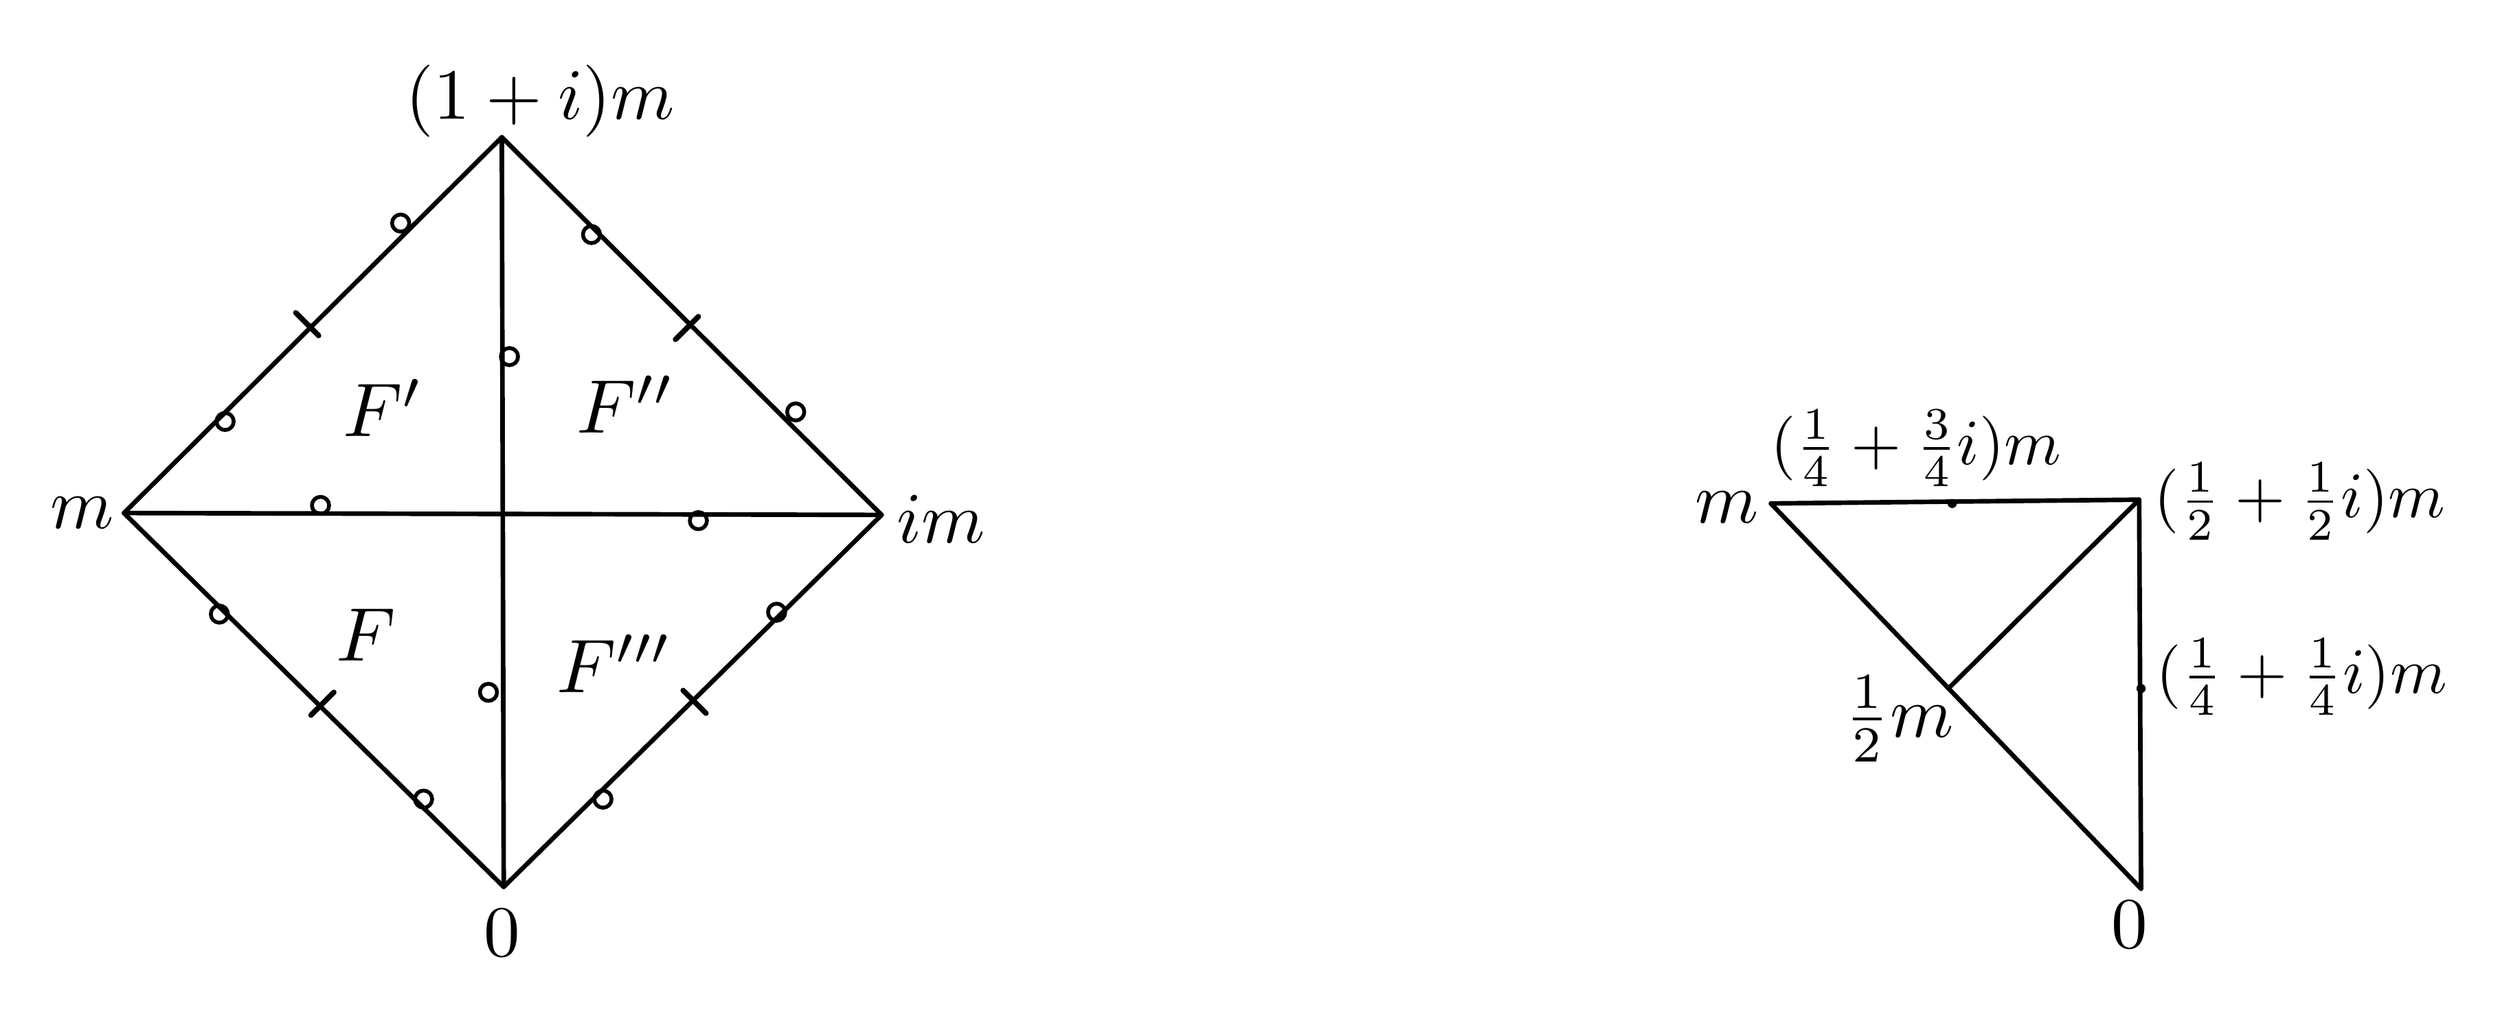
\begin{tikzpicture}[x=1bp,y=-1bp,line cap=round,line join=round]
\path[use as bounding box] (0,0) rectangle (1290,520);
\begin{pgfinterruptboundingbox}
\draw[line width=2.4bp] (55,259) -- (253,62) -- (452,260) -- (254,455) -- cycle;
\draw[line width=2.4bp] (253,62) -- (254,455);
\draw[line width=2.4bp] (55,259) -- (452,260);
\draw[line width=2bp] (108,211) circle[radius=4.5bp];
\draw[line width=2bp] (200,107) circle[radius=4.5bp];
\draw[line width=2bp] (300,113) circle[radius=4.5bp];
\draw[line width=2bp] (407,206) circle[radius=4.5bp];
\draw[line width=2bp] (105,312) circle[radius=4.5bp];
\draw[line width=2bp] (212,409) circle[radius=4.5bp];
\draw[line width=2bp] (397,311) circle[radius=4.5bp];
\draw[line width=2bp] (306,409) circle[radius=4.5bp];
\draw[line width=2bp] (158,255) circle[radius=4.5bp];
\draw[line width=2bp] (356,263) circle[radius=4.5bp];
\draw[line width=2bp] (257,177) circle[radius=4.5bp];
\draw[line width=2bp] (246,353) circle[radius=4.5bp];
\draw[line width=2.8bp] (145,154) -- (157,166);
\draw[line width=2.8bp] (344,168) -- (356,156);
\draw[line width=2.8bp] (153,365) -- (165,353);
\draw[line width=2.8bp] (348,352) -- (360,364);
\node[inner sep=0pt,outer sep=0pt,anchor=center] at (191,204) {\scalebox{4}{\ensuremath{F'}}};
\node[inner sep=0pt,outer sep=0pt,anchor=center] at (318,202) {\scalebox{4}{\ensuremath{F''}}};
\node[inner sep=0pt,outer sep=0pt,anchor=center] at (182,323) {\scalebox{4}{\ensuremath{F}}};
\node[inner sep=0pt,outer sep=0pt,anchor=center] at (312,338) {\scalebox{4}{\ensuremath{F'''}}};
\node[inner sep=0pt,outer sep=0pt,anchor=center] at (33,259) {\scalebox{3.8}{\ensuremath{m}}};
\node[inner sep=0pt,outer sep=0pt,anchor=center] at (273,43) {\scalebox{3.8}{\ensuremath{(1+i)m}}};
\node[inner sep=0pt,outer sep=0pt,anchor=center] at (483,262) {\scalebox{3.8}{\ensuremath{im}}};
\node[inner sep=0pt,outer sep=0pt,anchor=center] at (253,479) {\scalebox{3.8}{\ensuremath{0}}};
\draw[line width=2.4bp] (918,254) -- (1111,252) -- (1112,456) -- cycle;
\draw[line width=2.4bp] (1011,351) -- (1111,252);
\fill (1013,254) circle[radius=2.4bp];
\fill (1112,351) circle[radius=2.4bp];
\node[inner sep=0pt,outer sep=0pt,anchor=center] at (895,256) {\scalebox{3.8}{\ensuremath{m}}};
\node[inner sep=0pt,outer sep=0pt,anchor=center] at (994,225) {\scalebox{3.4}{\ensuremath{(\frac14+\frac34 i)m}}};
\node[inner sep=0pt,outer sep=0pt,anchor=west] at (1119,253) {\scalebox{3.4}{\ensuremath{(\frac12+\frac12 i)m}}};
\node[inner sep=0pt,outer sep=0pt,anchor=center] at (985,367) {\scalebox{3.8}{\ensuremath{\frac12 m}}};
\node[inner sep=0pt,outer sep=0pt,anchor=west] at (1120,345) {\scalebox{3.4}{\ensuremath{(\frac14+\frac14 i)m}}};
\node[inner sep=0pt,outer sep=0pt,anchor=center] at (1106,475) {\scalebox{3.8}{\ensuremath{0}}};
\end{pgfinterruptboundingbox}
\end{tikzpicture}
}\end{center}

% A544-P0328-D03
Zu $n$ sind zu rechnen alle Zahlen auf
\[
\text{der Linie }0\ldots\tfrac12m\qquad\text{Anzahl }=g
\]
Zu $n'$ alle Zahlen auf
\[
\text{der Linie }0\ldots(\tfrac14+\tfrac14i)m\qquad\text{Anzahl }=g'
\]
Zu $n''$ alle Zahlen innerhalb
\[
\text{des Dreiecks }\tfrac12m,m,(\tfrac12+\tfrac12i)m\qquad\text{Anzahl }=h
\]
Zu $n'''$ alle Zahlen innerhalb
\[
\text{des Dreiecks }0,\tfrac12m,(\tfrac12+\tfrac12i)m\qquad\text{Anzahl }=h'
\]
und ausserdem alle Zahlen auf
\[
\text{der Linie }(\tfrac14+\tfrac14i)m\dotstwo(\tfrac12+\tfrac12i)m\qquad\text{Anzahl }=g''
\]

% A544-P0328-D04
Man hat immer $g'+g''=g$, $aa+bb=p$, $\frac14(p-1)=g+g'+g''+h+h'$ Der Decident ist also
\SourceLeaf{329}%
% A544-P0329-D01
\[
D=S(0_{(+)},\tfrac12m,(\tfrac12+\tfrac12i)m_{(-)})+\tfrac12(p-1)+2g''
\]

% A544-P0329-D02
Man nehme nun an, dass für den Modulus $m+1+i$
\[
\begin{array}{clc}
g&\text{übergehe in}&G\\
g'&&G'\\
g''&&G''\\
h&&H\\
h'&&H'
\end{array}
\]
so hat man
\[
\begin{aligned}
&\Delta S(0_{(+)},\tfrac12m,(\tfrac12+\tfrac12i)m_{(-)})\\
&\quad=+S(0_{(+)},(\tfrac12+\tfrac12i)m,(\tfrac12+\tfrac12i)m+i_{(-)})\\
&\qquad-S(0_{(+)},\tfrac12m,\tfrac12m+\tfrac12+\tfrac12i_{(-)})\\
&\qquad-S(\tfrac12m,(\tfrac12+\tfrac12i)m,(\tfrac12+\tfrac12i)m+i,\ \tfrac12m+\tfrac12+\tfrac12i)
\end{aligned}
\]

% A544-P0329-D03
Das letzte dieser $S$ ist
\[
=\left[\tfrac12(a-b)\right]-\left[\tfrac12a\right]-S((\tfrac12+\tfrac12i)m,\tfrac12m,\tfrac12m+\tfrac12-\tfrac12i)
\]
wenn $a$ ungerade oder gerade
\[
\begin{aligned}
={}&\left[\tfrac12(a-b)\right]-\left[\tfrac12a\right]-S(-\tfrac12+\tfrac12i,\tfrac12m-\tfrac12+\tfrac12i,\tfrac12m+i)\\
={}&\left[\tfrac12(a-b)\right]-\left[\tfrac12a\right]+S(0_{(+)},\tfrac12m,\tfrac12m+\tfrac12+\tfrac12i_{(-)})\\
&-S(0_{(+)},(\tfrac12+\tfrac12i)m,(\tfrac12+\tfrac12i)m+i_{(-)})
\end{aligned}
\]

% A544-P0329-D04
Also
\[
\begin{aligned}
\Delta D={}&-\left[\tfrac12(a-b)\right]+\left[\tfrac12a\right]\\
&+2S(0_{(+)},(\tfrac12+\tfrac12i)m,(\tfrac12+\tfrac12i)m+i_{(-)})+a+b+1\\
&-2S(0_{(+)},\tfrac12m,\tfrac12m+\tfrac12+\tfrac12i_{(-)})-2g''+2G''
\end{aligned}
\]

% A544-P0329-D05
Die Bindezeichen gelten alle für den Fall, wo $a-b$ positiv ist, sonst nimmt man die entgegengesetzten.

% A544-P0329-D06
Wir zerlegen ferner $S(0_{(+)},(\frac12+\frac12i)m,(\frac12+\frac12i)m+i_{(-)})$ in
\[
\begin{aligned}
&S(0_{(+)},(\tfrac14+\tfrac14i)m,(\tfrac14+\tfrac14m)+\tfrac12i_{(-)})\\
&+\left[\tfrac12(a-b)\right]-\left[\tfrac14(a-b)\right]\\
&-S((\tfrac12+\tfrac12i)m_{(-)},(\tfrac14+\tfrac14i)m,(\tfrac14+\tfrac14i)m-\tfrac12i_{(-)})
\end{aligned}
\]

\SourceLeaf{330}%
% A544-P0330-D01
Der letzte Theil
\[
\begin{aligned}
={}&-S(\tfrac12+\tfrac12i_{(-)},(-\tfrac14-\tfrac14i)m+\tfrac12+\tfrac12i,\ (-\tfrac14-\tfrac14i)m+\tfrac12_{(+)})\\
={}&-S(-\tfrac12-\tfrac12i_{(-)},(\tfrac14+\tfrac14i)m-\tfrac12-\tfrac12i,\ (\tfrac14+\tfrac14i)m-\tfrac12_{(+)})\\
={}&-S(-\tfrac12-\tfrac12i_{(+)},(\tfrac14+\tfrac14i)m-\tfrac12-\tfrac12i,\ (\tfrac14+\tfrac14i)m-\tfrac12_{(-)})+g''-G''\\
={}&S(0_{(+)},(\tfrac14+\tfrac14i)m,(\tfrac14+\tfrac14i)m+\tfrac12i_{(-)})\\
&-S(0_{(+)},\tfrac12m,\tfrac12m+\tfrac12+\tfrac12i_{(-)})+g''-G''
\end{aligned}
\]

% A544-P0330-D02
Dadurch wird also
\[
\begin{aligned}
\Delta D={}&+\left[\tfrac12(a-b)\right]+\left[\tfrac12a\right]\\
&-4S(-\tfrac12-\tfrac12i_{(+)},\tfrac14+\tfrac14im-\tfrac12-\tfrac12i,\ (\tfrac14+\tfrac14i)m-\tfrac12_{(-)})\\
&-2\left[\tfrac14(a-b)\right]+a+b+1
\end{aligned}
\]

% A544-P0330-D03
Für den Fall der Vermehrung des Modulus um $1-i,-1+i,-1-i$ ist keine besondere Untersuchung nöthig, weil offenbar die Moduli $m,im,-m,-im$ gleiche Decidenten haben. Wir haben also folgende Lehrsätze:

% A544-P0330-D04
Ist der Decident des Modulus $a+bi,=D$, so sind die Decidenten von
{\small
\[
\begin{array}{l|l}
a+1+(b+1)i&D+a+b+1+[\tfrac12a]+[\tfrac12(a-b)]-2[\tfrac14(a-b)]\\
a+1+(b-1)i&D+a-b+1+[-\tfrac12b]+[-\tfrac12(a+b)]-2[-\tfrac14(a+b)]\\
a-1+(b+1)i&D-a+b+1+[\tfrac12b]+[\tfrac12(a+b)]-2[\tfrac14(a+b)]\\
a-1+(b-1)i&D-a-b+1+[-\tfrac12a]+[\tfrac12(b-a)]-2[\tfrac14(b-a)]
\end{array}
\]
}

% A544-P0330-D05
Hieraus ferner
{\footnotesize
\[
\begin{array}{l|l|l}
&&\begin{gathered}\text{oder insofern }a\text{ un-}\\\text{gerade ist}\end{gathered}\\
a+2+bi&\begin{aligned}D-\tfrac{a-b-3}2+2[\tfrac12a]&-2[\tfrac{a-b}4]\\&-2[\tfrac{-a-b-2}4]\end{aligned}&D+\tfrac{b-a-1}2\\[1ex]
a-2+bi&\begin{aligned}D+\tfrac{a-b+3}2+2[-\tfrac12a]&-2[\tfrac{b-a}4]\\&-2[\tfrac{a+b-2}4]\end{aligned}&D\\[1ex]
a+(b+2)i&\begin{aligned}D-\tfrac{a+b-3}2+2[\tfrac12b]&-2[\tfrac{a+b}4]\\&-2[\tfrac{a-b-2}4]\end{aligned}&D+\tfrac{a+b-3}2\\[1ex]
a+(b-2)i&\begin{aligned}D+\tfrac{a+b+3}2+2[-\tfrac12b]&-2[\tfrac{-a-b}4]\\&-2[\tfrac{b-a-2}4]\end{aligned}&
\end{array}
\]
}

% A544-P0330-D06
\[
\begin{array}{l|rl}
a+2+(b+2)i&2a-b+1+D&\text{oder }D+b-1\\
a+2+(b-2)i&-a-2b+1+D&D+a-1\\
a-2+(b+2)i&a+2b+1+D&D-a-1\\
a-2+(b-2)i&-2a+b+1+D&D-b-1
\end{array}
\]

